\lab{Intro to pandas II}{Intro to pandas II}
\label{lab:pandas4}
In this lab, we explore in further detail two specific areas where pandas can be a very useful tool:
analyzing sequential data, and working with large datasets that can't be stored entirely in memory.
\begin{warn}
This lab assumes pandas 0.14.0. Errors may occur if you have an earlier version.
You can check the version of pandas you are running by the following:
\begin{lstlisting}
>>> import pandas as pd
>>> pd.__version__
'0.14.0'
\end{lstlisting}
\end{warn}
\section*{Time Series Analysis}
A \emph{time series} is a particular type of data set that consists of a sequence of measurements or observations
generated at successive points in time. Examples include the yearly average temperate of a city, or
the price of a given stock measured daily.

\begin{comment}
This section needs beefing up. Topics to cover include:
    -using the date_range function to create dateTimeIndexes
    -showing different types of string reps that can be parsed, using format string to speed up parsing
    -resampling of a time series to change frequency levels.
    -slicing time series using date strings
    -the truncate method for time series
    -load in financial data, use some of the above techniques, do a fun, simple application.
\end{comment}

\section*{Working With Large Datasets}
In the real world, a data scientist is often confronted with large datasets that can't be held in memory all at once.
There are various solutions to this problem; in this section, we will explore how pandas uses the HDF5 file format
to allow us to work with datasets on disk.

HDF5, which stands for ``Hierarchical Data Format", is a data storage system especially suited for large numerical datasets.
Rich and efficient software libraries have been developed over the years to enable fast read and write operations,
which make HDF5 a competitive option for working with large datasets in many applications. The Python library pytables
is one such library, and the HDF5 capabilities in pandas are built directly on top of pytables.

We have two primary learning goals: how to get our data into the proper HDF5 format, and how to intelligently work with
the data once it's tidied up. Let's dive in.
\subsection*{Writing HDF5 Data}
The primary way we will interact with HDF5 data goes through the \li{HDFStore} object, which behaves somewhat like a dictionary.
To begin, let's instantiate such an object, and write data to it. Make sure to execute the code snippets throughout to ensure that
everything works as expected on your machine.
\begin{lstlisting}
>>> # we will create an HDFStore with the filename test_store.h5
>>> my_store = pd.HDFStore('test_store.h5')
>>> my_store
<class 'pandas.io.pytables.HDFStore'>
File path: test_store.h5
Empty
\end{lstlisting}
The file \li{'test_store.h5'} has just been created in your working directory, although it contains nothing as yet.
Write some pandas data to the store:
\begin{lstlisting}
>>> # instantiate data, write to store
>>> ts = pd.Series(index=['A', 'B', 'C', 'D'], data = np.random.randn(4))
>>> df = pd.DataFrame(index=range(6), columns=['a','b'], data=np.random.random((6,2)))
>>> my_store['ts'] = ts
>>> my_store['df'] = df
>>> my_store
<class 'pandas.io.pytables.HDFStore'>
File path: test_store.h5
/df            frame        (shape->[6,2])
/ts            series       (shape->[4]) 
\end{lstlisting}
Note the dict-like syntax for writing data to the store. We now see that the store contains two objects, which
can easily be retrieved in the following manner:
\begin{lstlisting}
>>> # retrieve the df from the store, check it is the same
>>> store_df = my_store['df']
>>> (df == store_df).all()
a    True
b    True
dtype: bool
\end{lstlisting}
Removing an object that you have written to the store can be accomplished as follows (although note that removing the
object doesn't necessarily free up space on the hard disk, so the file size may not decrease):
\begin{lstlisting}
>>> # let's remove the series ts
>>> del my_store['ts'] # or my_store.remove('ts')
>>> my_store
<class 'pandas.io.pytables.HDFStore'>
File path: test_store.h5
/df            frame        (shape->[6,2])
\end{lstlisting}

The read and write operations that we have explored so far work just fine for small objects that can fit entirely in memory,
but the story is different when it comes to writing large datasets to an HDF5 file. Suppose we have a CSV file containing the
large dataset that we want to work with. One basic approach to storing this data in HDF5 format is to read and write it by 
\emph{chunks}, that is, move the data into an HDF5 store a few lines at a time. This ensures that we never have to read too much
of the data into memory at once. 

The \li{read_csv} function in pandas allows for reading a file by chunks of rows. We simply need to specify the keyword argument
\li{chunksize}, which gives the number of rows of the file to read in each time. Most other pandas data readers have a similar
option for loading data by chunks. It is also important to specify the correct data types of each column when reading in the chunks
of data. This will ensure that a consistent data type is used when writing to the HDF5 store. To do this, create a dict that
maps each column name to its correct data type. Columns containing strings should have the \li{object} datatype, and columns
containing numerical data may be ints or floats. Any column that contains date data should NOT be included in the dictionary,
but rather should be passed as the \li{parse_dates} keyword argument (a list of the column names containing dates). 

To iteratively write data to a single object in an HDF5 store, we must use the \li{append} method. This will store the data in a 
particular format called a \emph{table}, an on-disk data structure geared toward efficient querying of the rows. There are a few
parameters that we must tune in order to write the data successfully.
\begin{itemize}
\item \li{key}: This is the target object in the HDF5 store to which we want to write. 
\item \li{value}: This is the actual chunk of data (such as a \li{DataFrame}) that we want to append to the store.
\item \li{data_columns}: A list of the column names of the incoming data that should be indexed. You should include all 
columns that you will use in subsequent queries of the data. For example, if my dataset has a column labeled `A', and I anticipate
wanting to select all rows where the value in column `A' is greater than, say, 0, then it is imperative that \li{data_columns} includes
`A'. Try to avoid including columns that aren't needed in the queries, as performance can decrease with a larger number of indexed
columns. This argument only needs to be specified for the \emph{first} chunk to be written.
\item \li{min_itemsize}: This is an int that specifies the maximum length of a string found in the dataset. If you are unsure of the 
exact length of the longest string, try setting this to a high default value (say 100). If you attempt to write data containing 
a string whose length exceeds \li{min_itemsize}, an error is raised. This argument is also only required for the first chunk.
\item \li{index}: This argument is a boolean flag that indicates whether the data should be indexed as it is written. By setting
\li{index=False}, the data is written much faster.
\end{itemize}
In the code below, we create a CSV file containing toy data, then write it by chunks to our HDF5 store.
\begin{lstlisting}
>>> # first create the toy CSV file
>>> n_rows = 10000
>>> n_cols = 3
>>> csv_path = 'toy_data.csv'
>>> csv_file = open(csv_path, 'w')
>>> csv_file.write("A B C\n")
>>> for i in xrange(n_rows):
>>>     for num in np.random.randn(3):
>>>         csv_file.write(' ' + str(num))
>>>     csv_file.write('\n')
>>> csv_file.close()

>>> # now iteratively write the data to the store
>>> n_chunk = 1000
>>> col_types = {'A':np.float, 'B':np.float, 'C':np.float}
>>> reader = pd.read_csv(csv_path, sep=' ', dtype=col_types, index_col=False, chunksize=n_chunk, skipinitialspace=True)
>>> first = True # a flag for the very first chunk
>>> data_cols=['B', 'C'] # queries involving cols B and C will be allowed
>>> for chunk in reader:
>>>     if first:
>>>         my_store.append('toy_data', chunk, data_columns=data_cols, index=False)
>>>         first = False
>>>     else:
>>>         my_store.append('toy_data', chunk, index=False)
>>> my_store
<class 'pandas.io.pytables.HDFStore'>
File path: test_store.h5
/df                  frame        (shape->[6,2])
/toy_data            frame_table  (typ->appendable,nrows->10000,ncols->3,indexers->[index],dc->[B,C])
\end{lstlisting}
If an error of any type occurs when writing your data, and you need to start over, it is necessary to remove
the previously written data, since the \li{append} function doesn't overwrite existing data.

Now that the data is in the HDF5 store, we should index the table, which can speed up query operations.
This is done as follows:
\begin{lstlisting}
>>> my_store.create_table_index('toy_data', optlevel=9, kind='full')
\end{lstlisting}
Obviously the toy data in this example is small enough to fit in memory, but it illustrates a basic approach
to moving large datasets into a HDF5 store.

\begin{problem}
Write the data contained in the file \li{campaign.csv} to an HDF5 store using the chunking approach.
We recommend setting the \li{chunksize} argument to 50,000. There will be just over 100 chunks for this
chunk size, so you can track your progress by printing out a counter, if you wish. The whole writing
process will likely take a few minutes.

The file \li{campaign_format.txt} contains information about the dataset, including the column names and descriptions.
Consult this file and note which, if any, columns contain date information. Use this information to appropriately
set the \li{parse_dates} argument in the \li{read_csv} function. This argument should be a list of the column names
that include date information. Note also that some of the columns contain strings, so remember the 
\li{min_itemsize} argument. Finally, you will be analyzing this data in the remainder of the lab, so glance over 
the problems below to determine which columns need to be indexed. 

Once you have finished writing to the store, create a table index for the data, just as shown in the example above.
\end{problem}

\subsection*{Working With On-Disk Arrays}
Now that we have the data in a HDF5 table, how do we work with it? The key here is to only read in subsets
of the data, since trying to read the entire dataset at once may result in swamping the memory and crashing
the system. The \li{select} method allows us to do just this. It takes two basic arguments: first, the name
of the table in the store that we want to query, and second, a query statement. Remember, the 
query statement may not reference columns that weren't included in \li{data_columns}.
\begin{lstlisting}
>>> # this query is OK
>>> my_store.select('toy_data', where = ["'B' < 0", "'C' > 0"])

>>> # this query is NOT OK
>>> my_store.select('toy_data', where = ["'A' < .5"])
\end{lstlisting}
Note that each logical statement in the \li{where} list is combined with a logical AND.

Let's look at some simple examples with our campaign dataset. We assume that the data is in a HDF5 store called 
\li{store}. Follow along to make sure you get the same results.
\begin{lstlisting}
>>> # get a list of the candidates; result should be 14 candidates
>>> cands = store.select_column('campaign', 'cand_nm').unique()

>>> # find number of contributions from UT
>>> n_UT = len(store.select('campaign',where = ["'contbr_st' == 'UT'", "columns='contbr_st'"]))
>>> n_UT
50462

>>> # find number of UT contributions to Romney
>>>  n_rom_UT = len(store.select('campaign', where = ["'contbr_st' == 'UT'", "'cand_nm'=='Romney, Mitt'", "columns='contbr_st'"]))
>>> n_rom_UT
26962

>>> # proportion of UT contributions that went to Romney
>>> np.float(n_rom_UT)/n_UT
0.534303039911
\end{lstlisting}

\begin{problem}
How many contributors in California gave to Obama? To Romney?
\end{problem}

It is also possible to execute more complicated queries involving grouping operations, although some care is required.
Consider the following question: how many contributions came from each state, and what is the average contribution
from each state? To answer this question, we need to aggregate information grouped by each state. If we could hold
the data in memory, we could use a simply \li{groupby} operation, but since our data resides on disk, the solution is
a bit more involved. Fortunately, the \li{'contbr_st'} column alone is small enough to load into memory, so we do that.
We can then utilize the \li{Series} method \li{value_counts}, which counts the number of occurrences of each distinct
value in the column. In this way, we obtain a \li{Series} indexed by the states, and containing the number of 
contributions from each state.
\begin{lstlisting}
>>> # load in the state column, then calculate the counts
>>> states = store.select_column('campaign','contbr_st')
>>> states = states.value_counts()
\end{lstlisting} 
Next, we want to iterate through each state, and calculate the mean contribution.
\begin{lstlisting}
>>> st_contb = []
>>> for state in states.index:
>>>     grp = store.select('campaign', where=["'contbr_st'=\"{}\"".format(state), "columns='contb_receipt_amt'"])
>>>     st_contb.append(grp['contb_receipt_amt'].mean())
\end{lstlisting}
To tidy up our results, we create a \li{DataFrame} indexed by the state, containing the number of contributions
and average contribution. Then we plot top results.
\begin{lstlisting}
>>> state_info = pd.DataFrame({'Count':states, 'Avg Contb':st_contb})
>>> state_info.sort(columns='Count', ascending=False, inplace=True)
>>> plt.subplot(211)
>>> state_info['Count'][:10].plot(kind='bar')
>>> plt.subplot(212)
>>> state_info['Avg Contb'][:10].plot(kind='bar')
>>> plt.show()
\end{lstlisting}
Results are shown in Figure \ref{pandas:states}
\begin{figure}
\centering
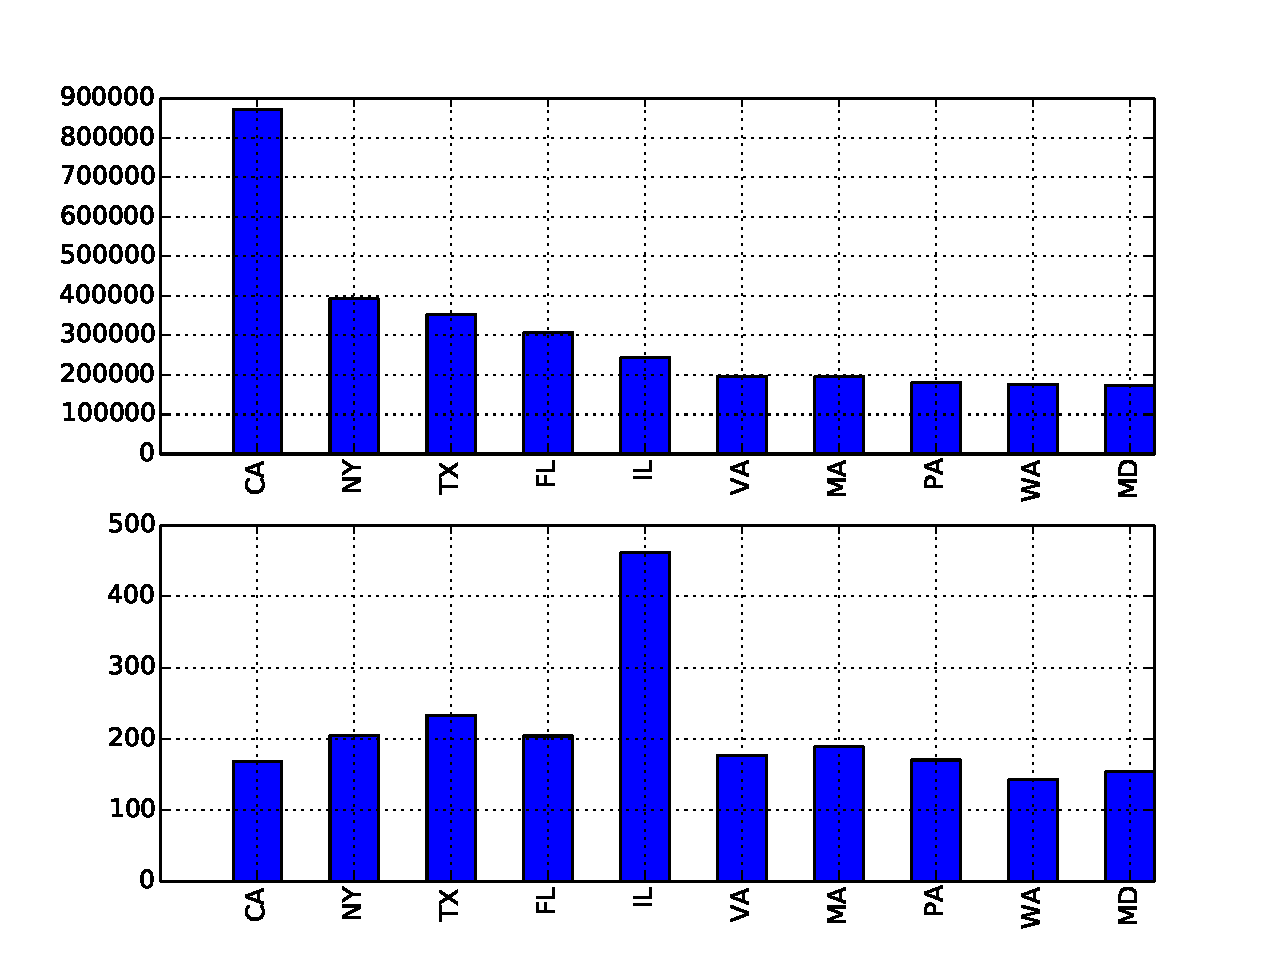
\includegraphics[width=\textwidth]{states.pdf}
\caption{Top 10 contributing states (top), and their average contributions (bottom).}
\label{pandas:states}
\end{figure}

\begin{problem}
Calculate the total net contributions to each candidate, and plot the results in a bar graph.
Your result should match Figure \ref{pandas:cand_contb}.
\end{problem}

\begin{figure}
\centering
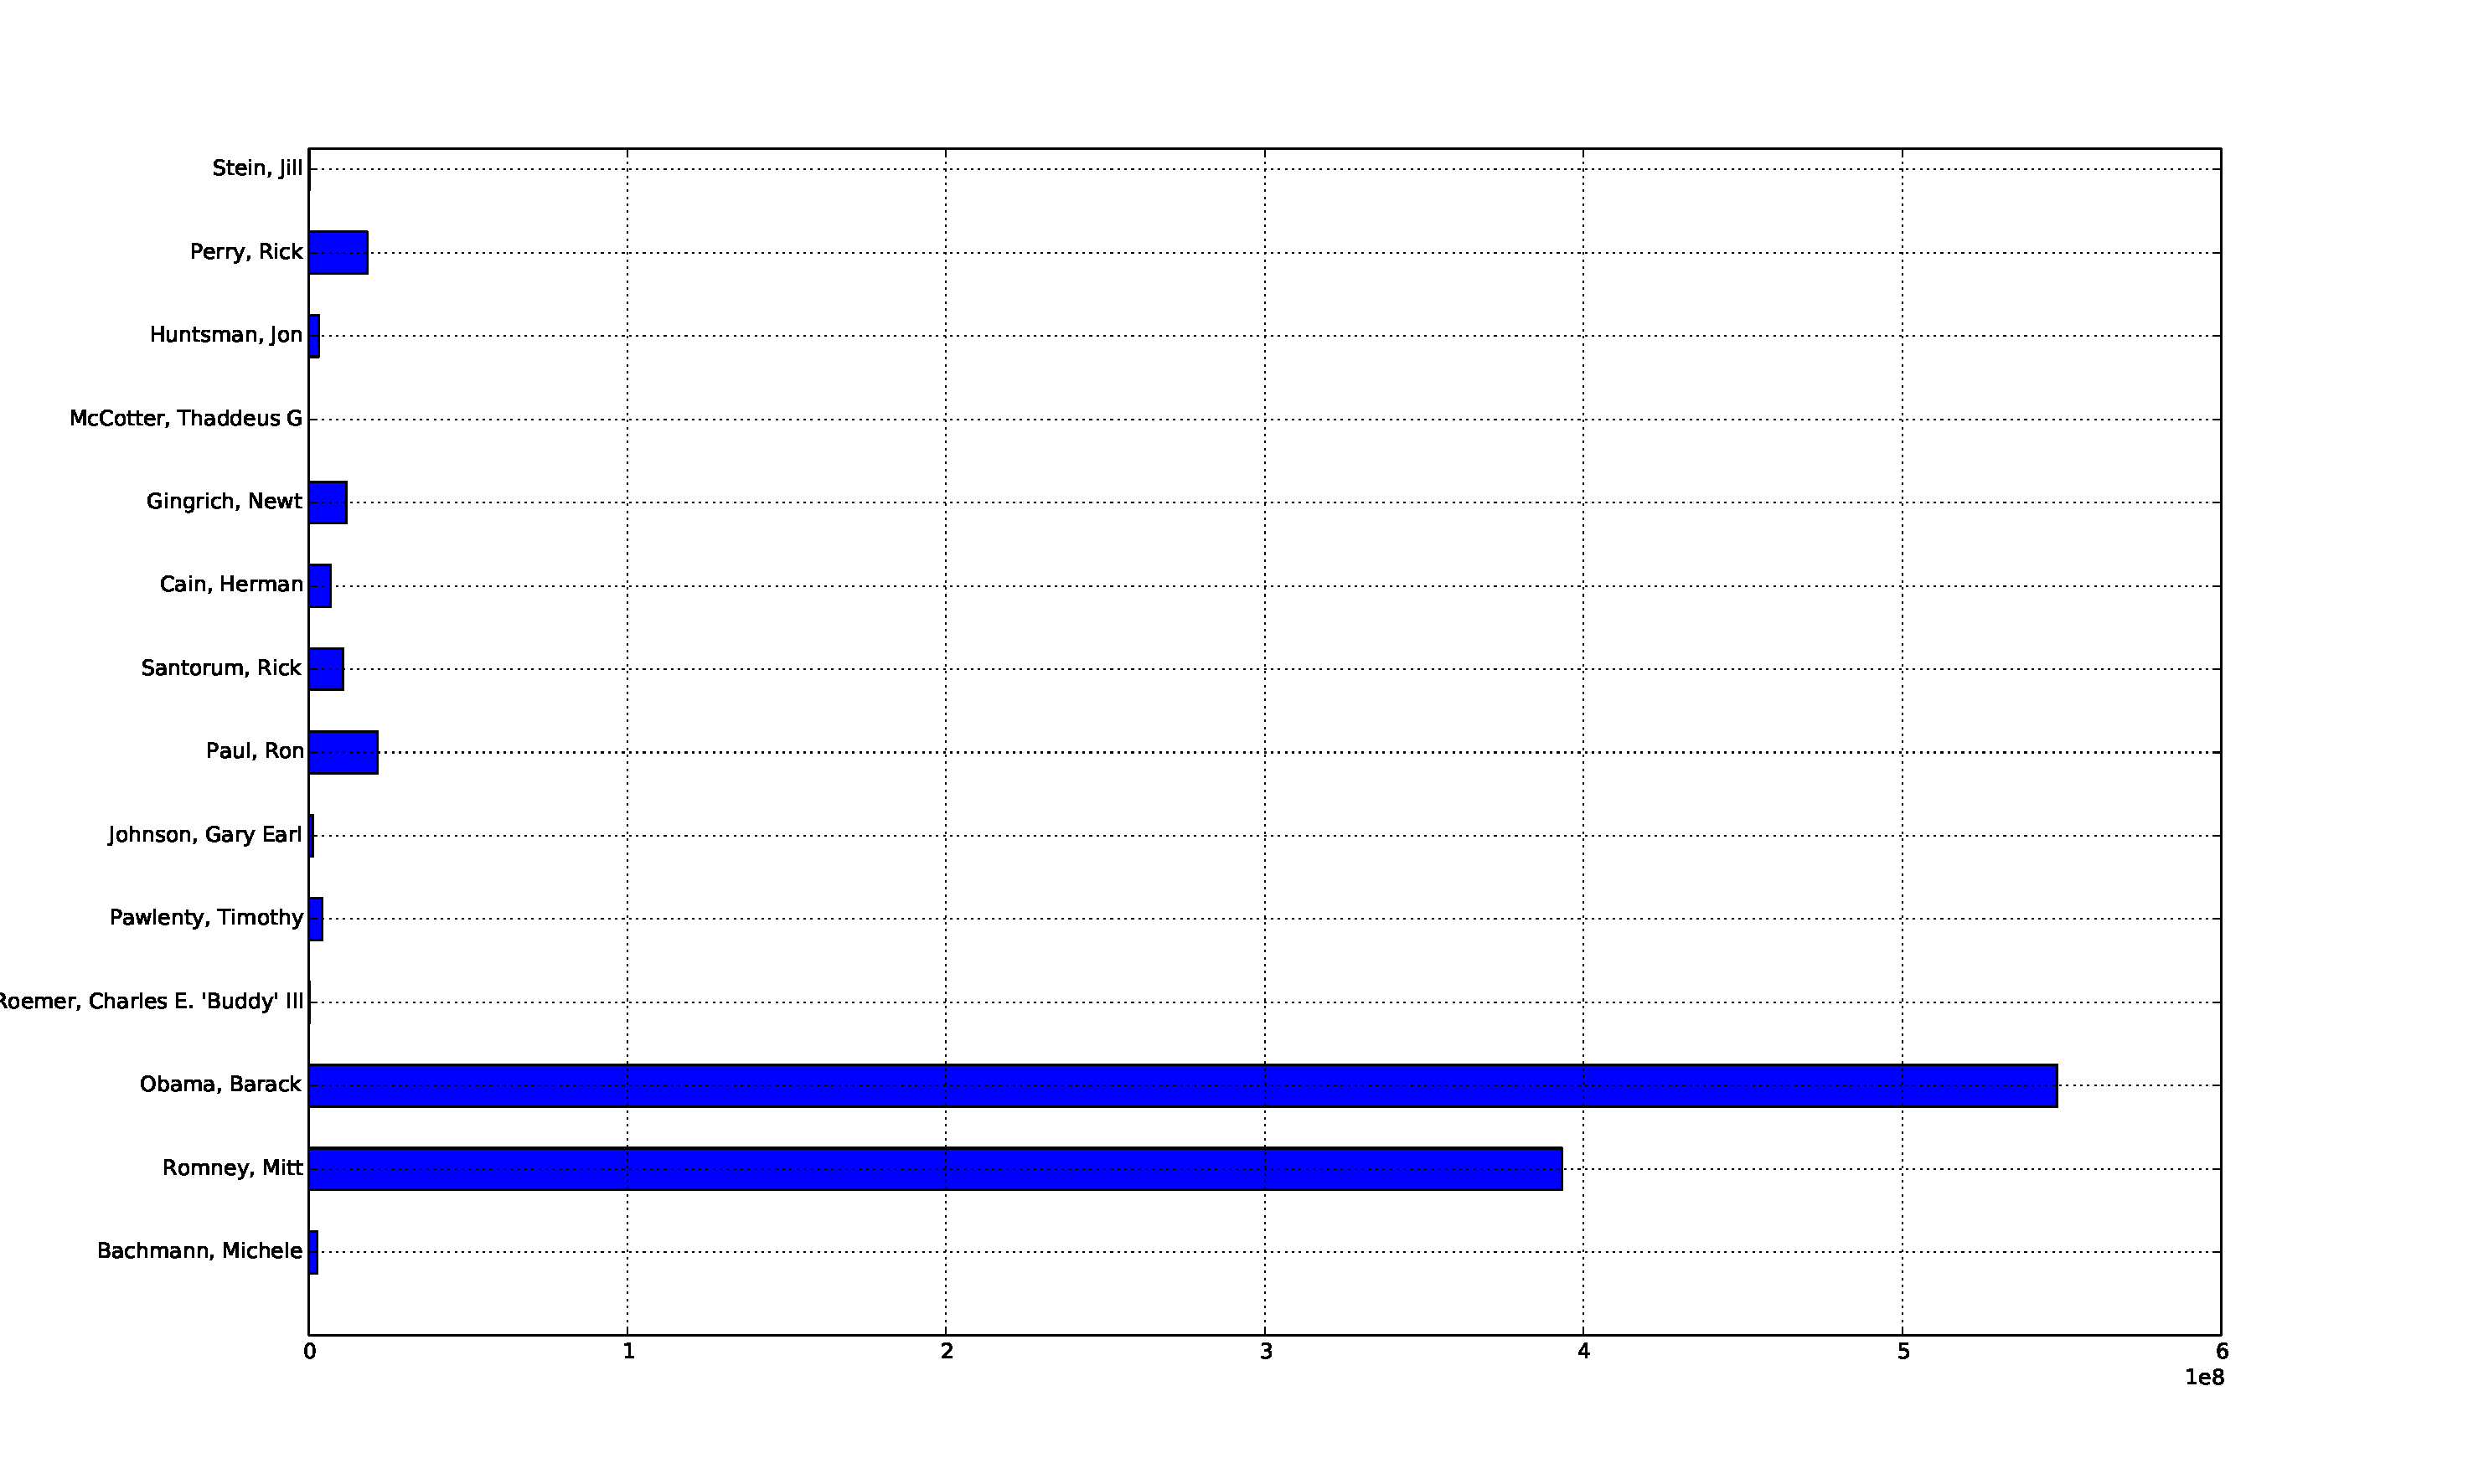
\includegraphics[width=\textwidth]{cand_contb.pdf}
\caption{Total net contributions to each candidate.}
\label{pandas:cand_contb}
\end{figure}


\begin{problem}
Calculate the frequency of the 20 most common occupations of contributors in the dataset. 
Also calculate the average positive contribution amount for each of these 20 occupations.
Plot the results in two bar graphs. You results should match Figure \ref{pandas:occupation}.
\end{problem}

\begin{figure}
\centering
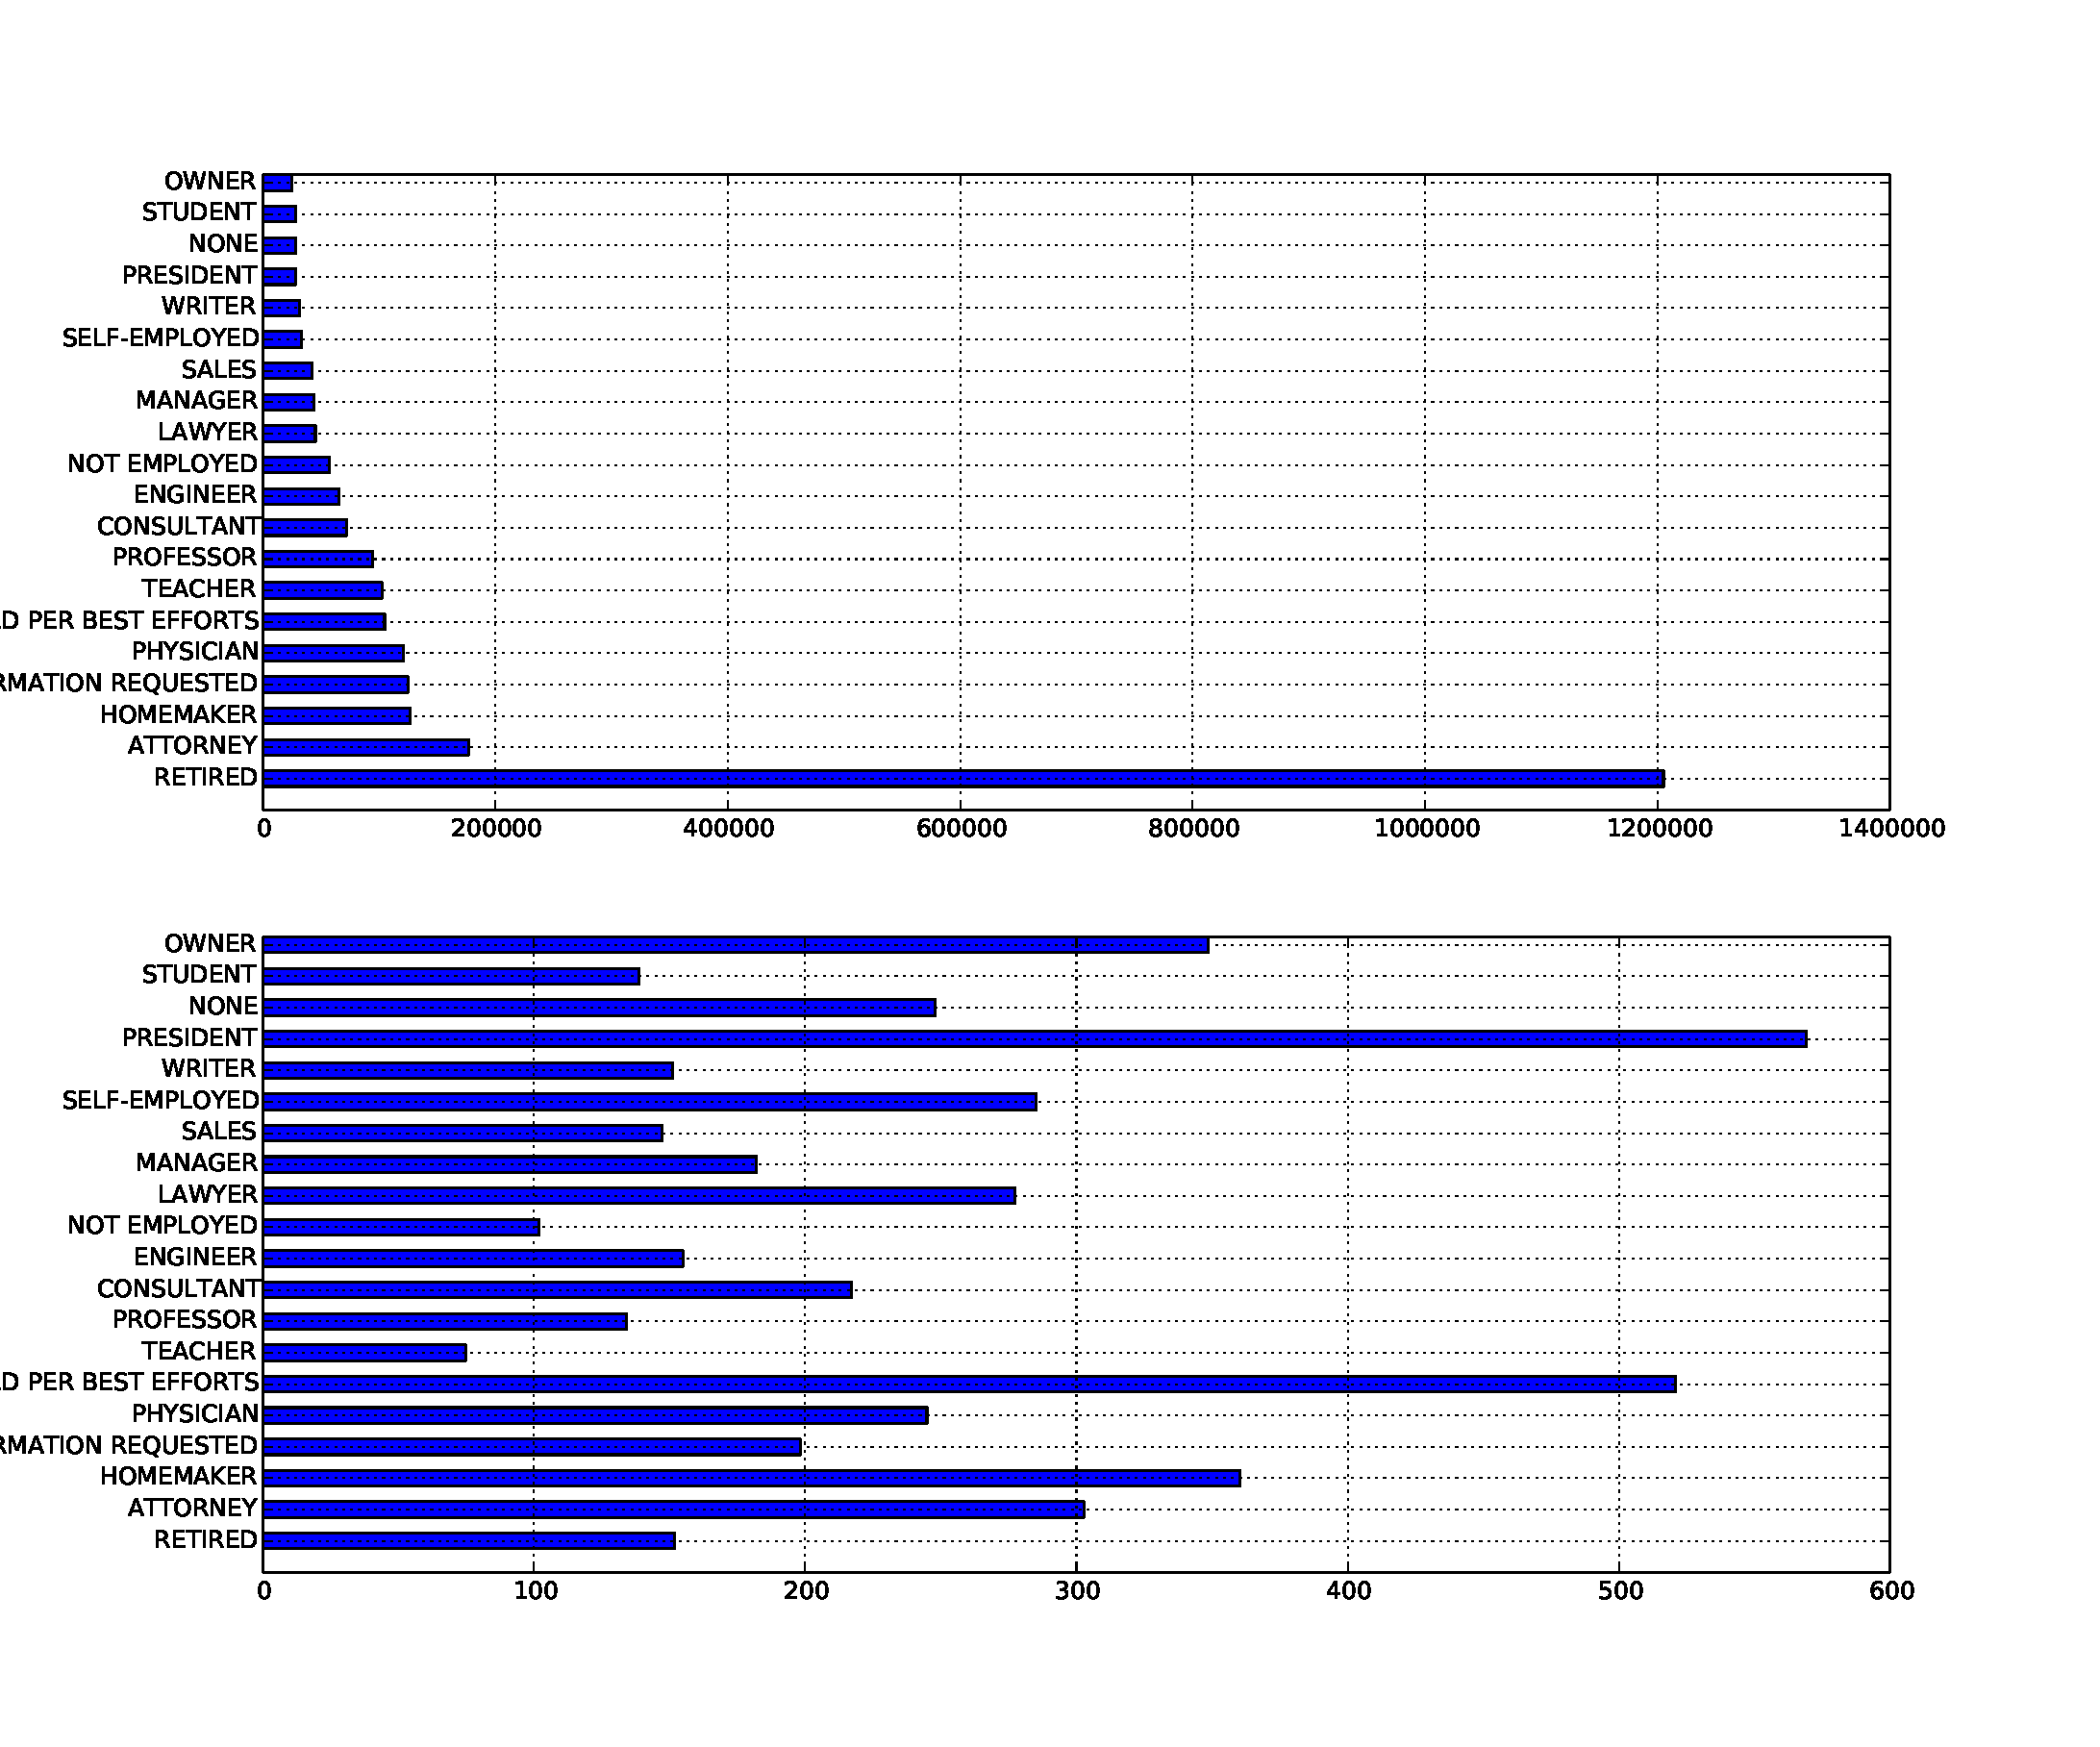
\includegraphics[width=\textwidth]{occupation.pdf}
\caption{Top 20 occupations of contributors (above) and average contribution of each
occupation (below).}
\label{pandas:occupation}
\end{figure}

What if you are interested in the contributions to a candidate as a function of time?
Let's first aim to create a \li{DataFrame} containing the contribution amount and date for
all contributions going to Ron Paul.
\begin{lstlisting}
>>> cand = 'Paul, Ron'
>>> cand_contb = store.select('campaign', where=["'cand_nm'==\"{}\"".format(cand)])[['contb_receipt_amt', 'contb_receipt_dt']]
\end{lstlisting}
Next, we need to group by date, and apply the sum function to add up contributions for each particular date.
This can be done with the \li{groupby} function as follows:
\begin{lstlisting}
>>> contb = cand_contb.groupby(by='contb_receipt_dt').sum()
\end{lstlisting}
Plotting this time series yields Figure \ref{pandas:paul}.

\begin{figure}
\centering
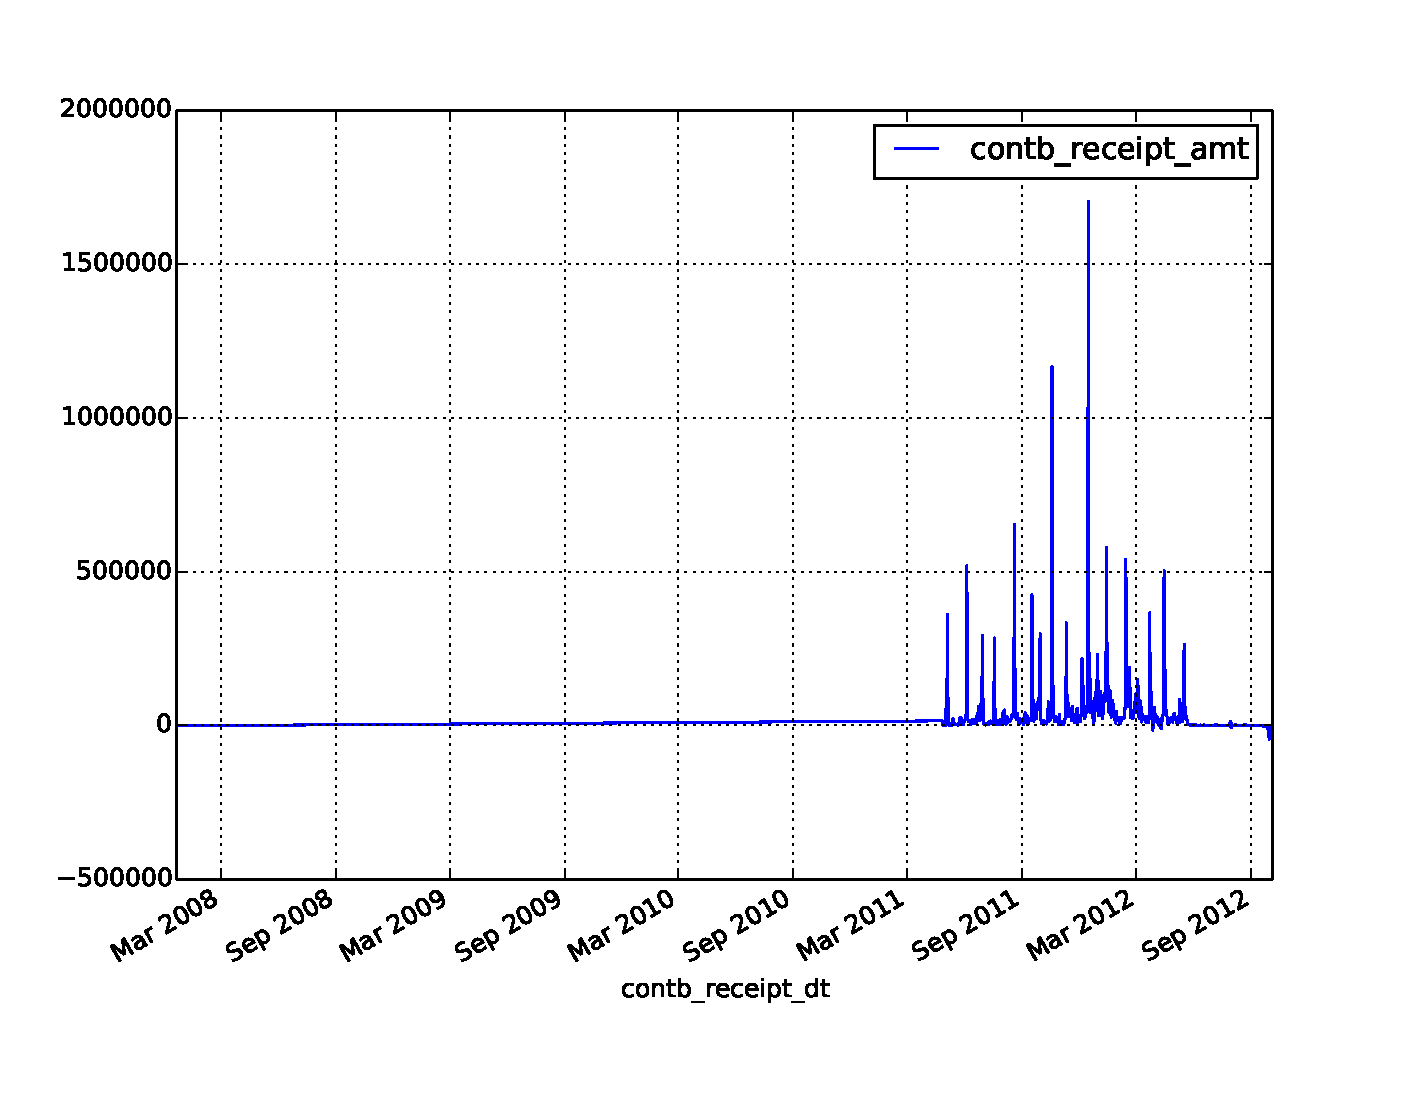
\includegraphics[width=\textwidth]{paul.pdf}
\caption{Campaign Contributions to Ron Paul over time.}
\label{pandas:paul}
\end{figure}

\begin{problem}
Plot the running total of campaign contributions as a function of time
for Mitt Romney, Barack Obama, and Newt Gingrich (all on the same graph). 
Your results should match Figure \ref{pandas:cand_time}.
\end{problem}
\begin{figure}
\centering
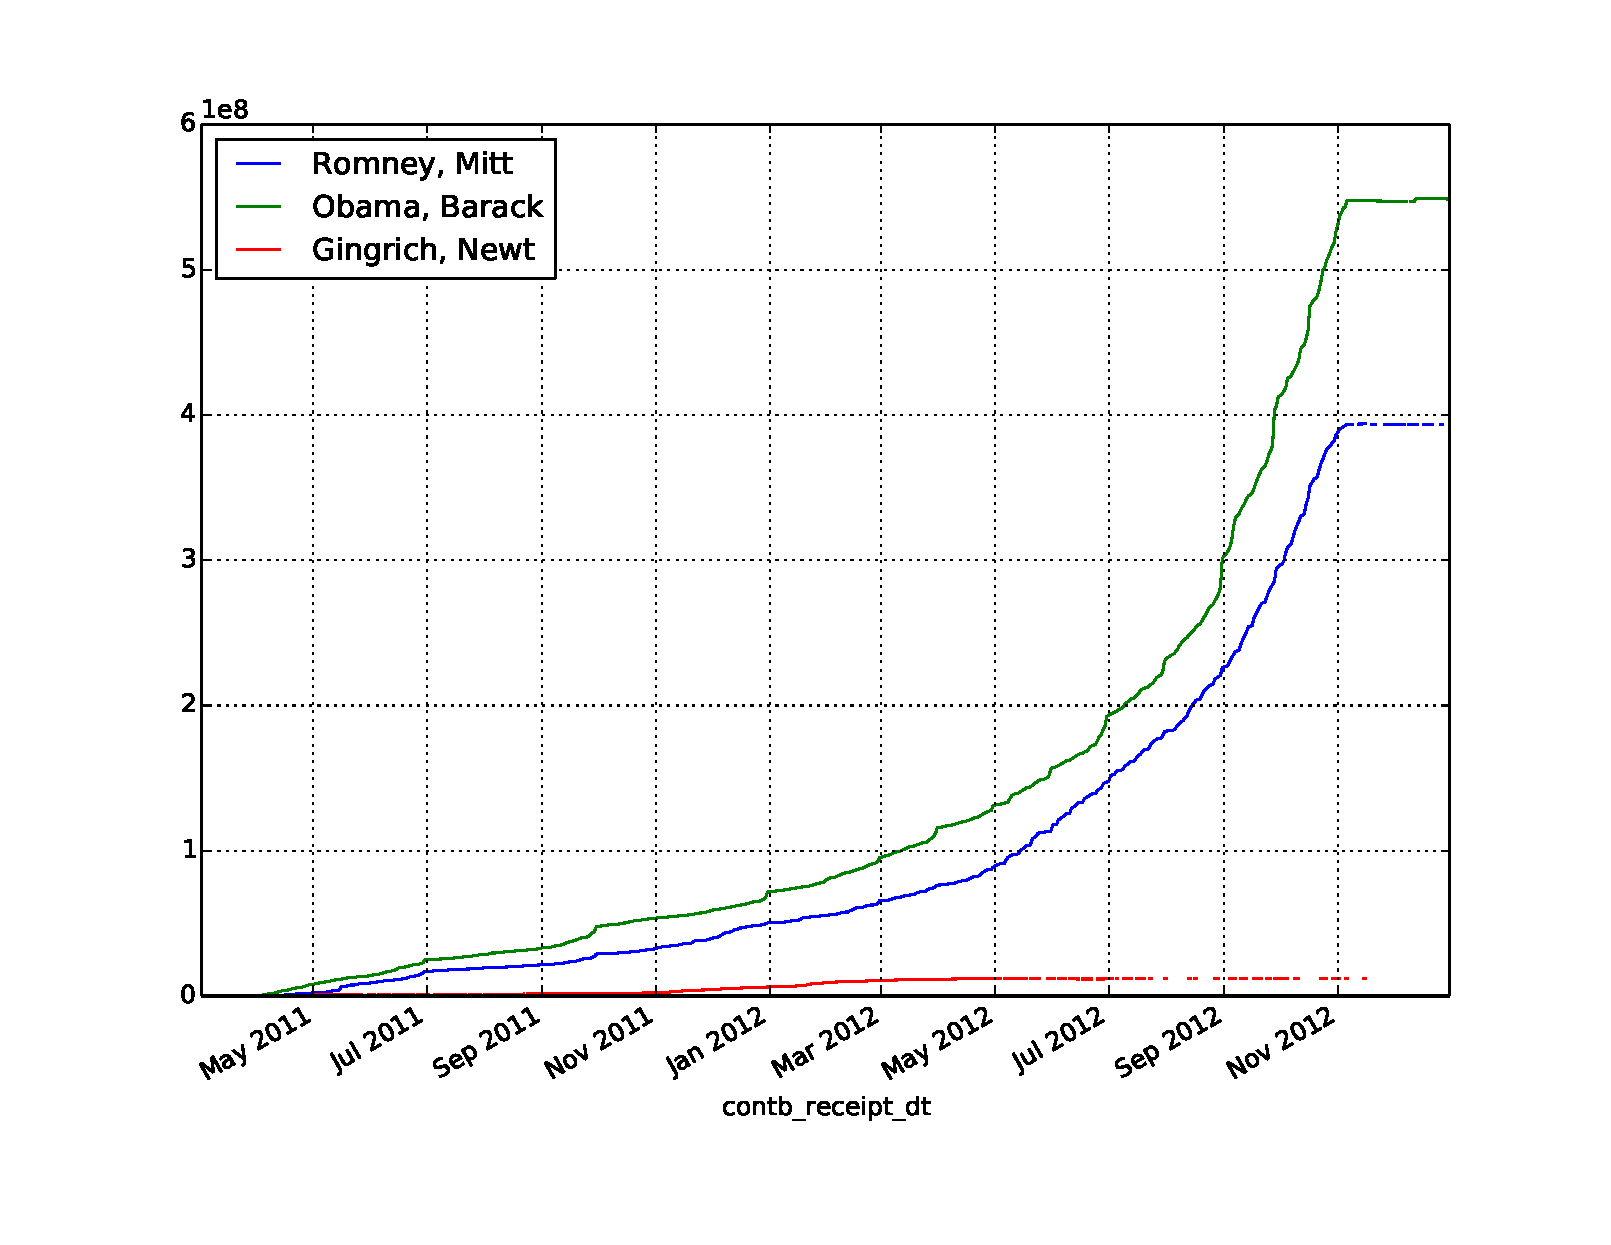
\includegraphics[width=\textwidth]{cand_time.pdf}
\caption{Running contribution totals for three candidates.}
\label{pandas:cand_time}
\end{figure}

Each data project brings with it a new set of problems and pitfalls, but a careful application of the principles 
in this lab will provide a good starting point for working with large datasets in pandas.
